\subsection{运行完整性与固定参数}
实验在Windows11、Intel Core i9-12900H和RTX3070Ti Laptop GPU（8192MiB）上运行，CPU线程数为1。
环境为Python3.12.4、PyTorch2.7.1+cu128、CUDA12.8，显卡驱动591.74。
正式清单中45次矩阵运行、9次语言模型运行全部完成，每组均为三个独立种子。校准和学习率筛选未计入正式样本。
GPU共享账本累计58.46分钟，包含校准、筛选、训练、测试评估，以及一次测量维护重启的保守记账；预算上限为480分钟。
重启发生在调参阶段，检查点与中断原因保留，正式配置和目标步数未因此改变。
依据预先规定的1.3倍耗时预测规则，正式长度固定为2000步，即每次处理8,192,000字节。
语言模型选定的学习率为AdamW 0.001、Muon 0.02；辅助AdamW为$3\times10^{-4}$。
三种正式方法均使用微批8、累积4。

\subsection{矩阵优化结果}
表\ref{tab:matrix}给出1000步后的目标值，已知最优值为零。$\pm$表示样本标准差，时间列为三次任务累计墙钟时间的均值。
在本次固定步长和搜索网格下，三个条件数中AdamW的终点目标值均更低。
例如条件数100时，AdamW为$0.0173\pm 0.00227$，NS5为$0.266\pm 0.0346$。
这并不与驻点定理矛盾：本实验采用固定经验步长，而定理按总时域设置参数，且没有给出算法之间的无条件优越性。
\begin{table}[htbp]\centering\small
\caption{矩阵正式实验终点目标值，$n=3$}\label{tab:matrix}
\begin{tabular}{rlrr}\toprule 条件数&方法&目标值（均值$\pm$标准差）&时间/s\\\midrule
1 & AdamW & $0.000179\pm 1.26\times10^{-6}$ & 0.595 \\
1 & Muon-SVD & $0.0083\pm 0.00283$ & 0.786 \\
1 & Muon-NS1 & $0.00399\pm 0.00369$ & 0.674 \\
1 & Muon-NS3 & $0.00331\pm 0.00226$ & 0.866 \\
1 & Muon-NS5 & $0.00528\pm 0.00286$ & 1.048 \\
10 & AdamW & $0.00204\pm 0.000129$ & 0.590 \\
10 & Muon-SVD & $0.0348\pm 0.00632$ & 0.781 \\
10 & Muon-NS1 & $0.0178\pm 0.00096$ & 0.657 \\
10 & Muon-NS3 & $0.0352\pm 0.00656$ & 0.853 \\
10 & Muon-NS5 & $0.0299\pm 0.00547$ & 1.030 \\
100 & AdamW & $0.0173\pm 0.00227$ & 0.598 \\
100 & Muon-SVD & $0.206\pm 0.00101$ & 0.771 \\
100 & Muon-NS1 & $0.122\pm 0.00182$ & 0.666 \\
100 & Muon-NS3 & $0.322\pm 0.0277$ & 0.842 \\
100 & Muon-NS5 & $0.266\pm 0.0346$ & 1.033 \\
\bottomrule\end{tabular}\end{table}

\begin{figure}[htbp]\centering
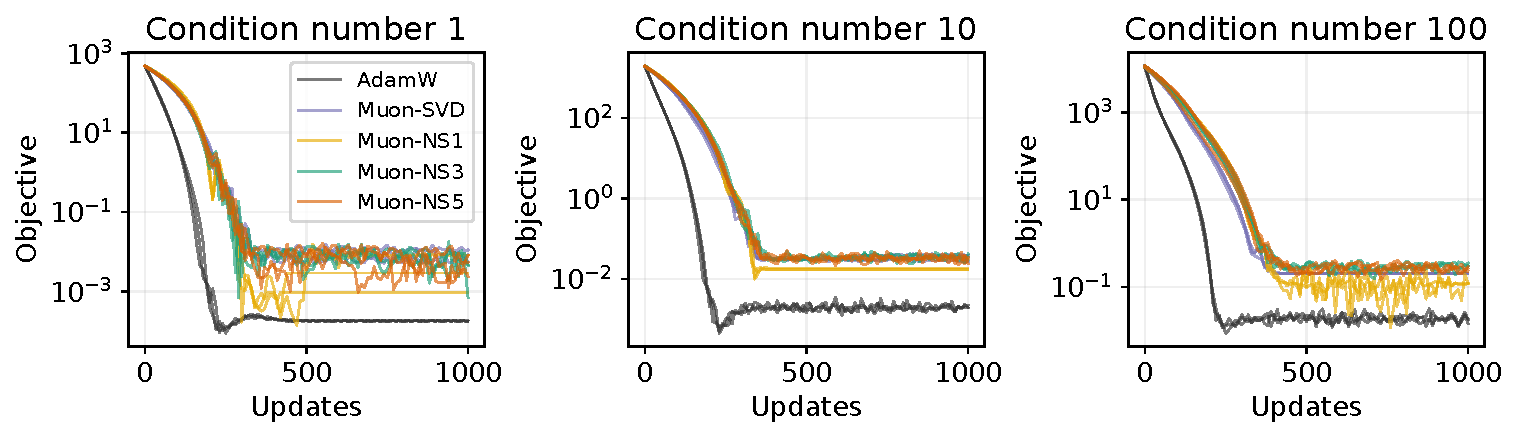
\includegraphics[width=\linewidth]{figures/matrix_objective.pdf}
\caption{矩阵目标值轨迹。每条线对应一个种子；纵轴为对数坐标。}\label{fig:matrix}
\end{figure}
\begin{figure}[htbp]\centering
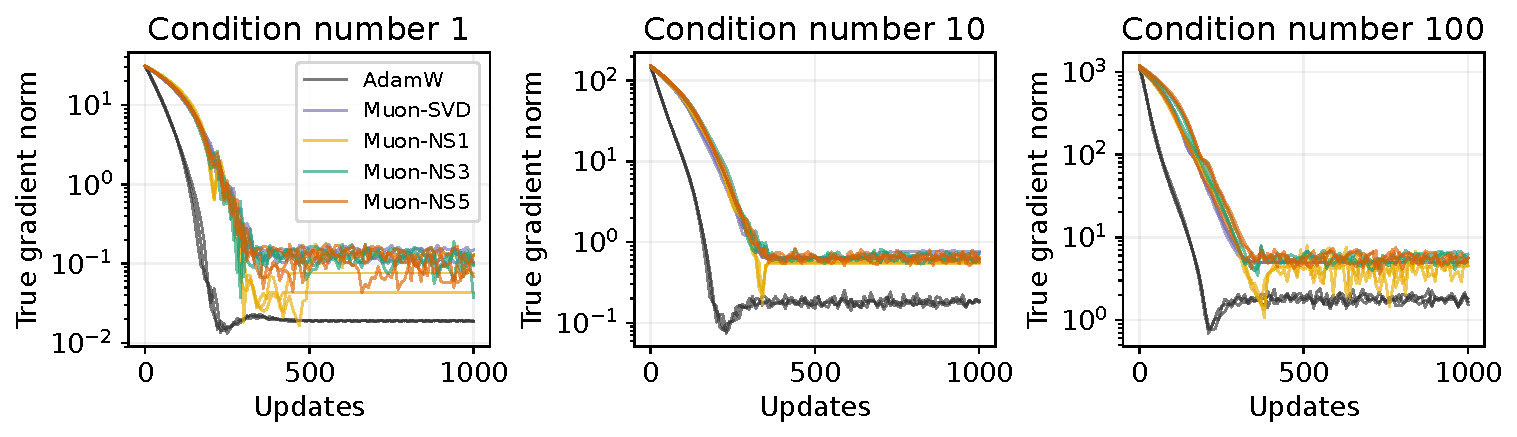
\includegraphics[width=\linewidth]{figures/matrix_gradient.pdf}
\caption{真实梯度Frobenius范数。该指标从解析梯度计算，未用优化器内部动量替代。}
\end{figure}
图\ref{fig:matrix}显示了下降与终点邻域的行为。极因子类方向改变梯度幅值信息，固定步长在接近解时仍可能产生非消失更新；这是解释终点差异的一种机制，本文没有额外实验把它识别为唯一原因。
两个方法的矩阵学习率都在搜索网格上界处选中，因而本次筛选没有定位各自全局最优学习率。

\begin{figure}[htbp]\centering
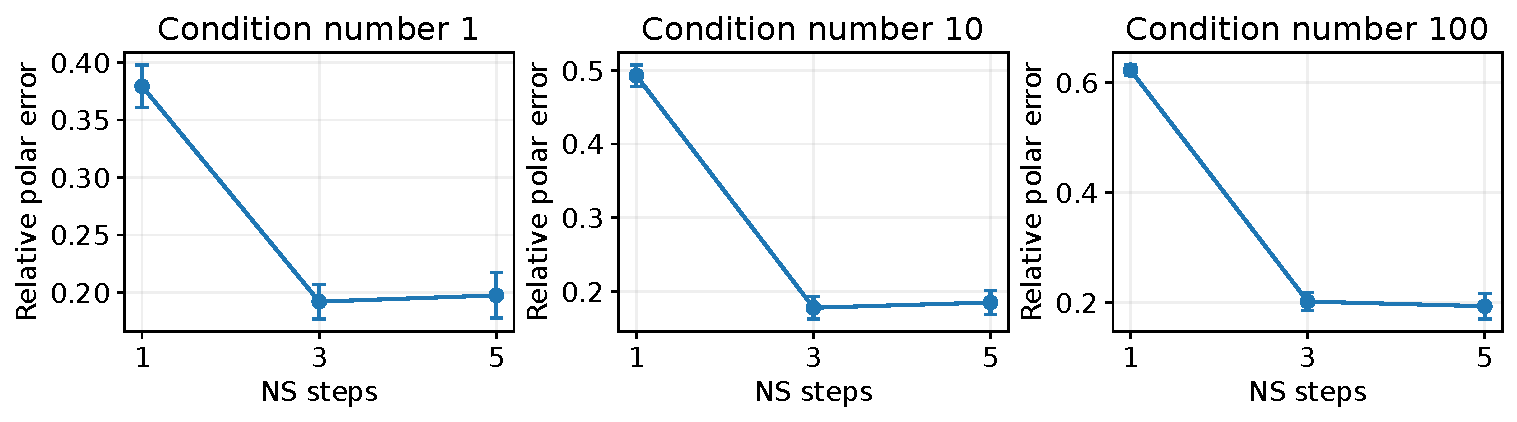
\includegraphics[width=\linewidth]{figures/ns_diagnostics.pdf}
\caption{同一初始梯度输入下，NS输出相对紧致SVD极因子的Frobenius误差。误差条为三个输入种子的样本标准差。}\label{fig:ns}
\end{figure}
图\ref{fig:ns}将近似误差与完整优化轨迹分开。误差与最终损失不是同一指标；有限步经验多项式的正向对齐也不要求极因子误差逐步趋零。

\subsection{小型语言模型结果}
表\ref{tab:language}中验证损失来自相同总训练字节预算的终点，测试损失来自各次运行由验证集选出的最佳检查点。
二者可能对应不同步数，不能把测试结果解释为终点模型的测试损失。所有损失单位均为nats/byte。
\begin{table}[htbp]\centering\small
\caption{语言模型正式实验，$n=3$；时间为任务累计墙钟均值，显存为峰值已分配量均值}\label{tab:language}
\resizebox{\linewidth}{!}{\begin{tabular}{lrrrr}\toprule
方法&终点验证损失&最佳模型测试损失&时间/s&显存/MiB\\\midrule
AdamW & $1.4766\pm 0.0071$ & $1.6073\pm 0.0100$ & 295.6 & 199.1 \\
Muon-NS5 & $1.4329\pm 0.0008$ & $1.5626\pm 0.0056$ & 349.2 & 181.1 \\
Muon-NS3 & $1.4315\pm 0.0027$ & $1.5580\pm 0.0102$ & 369.2 & 181.1 \\
\bottomrule\end{tabular}}\end{table}

\begin{figure}[htbp]\centering
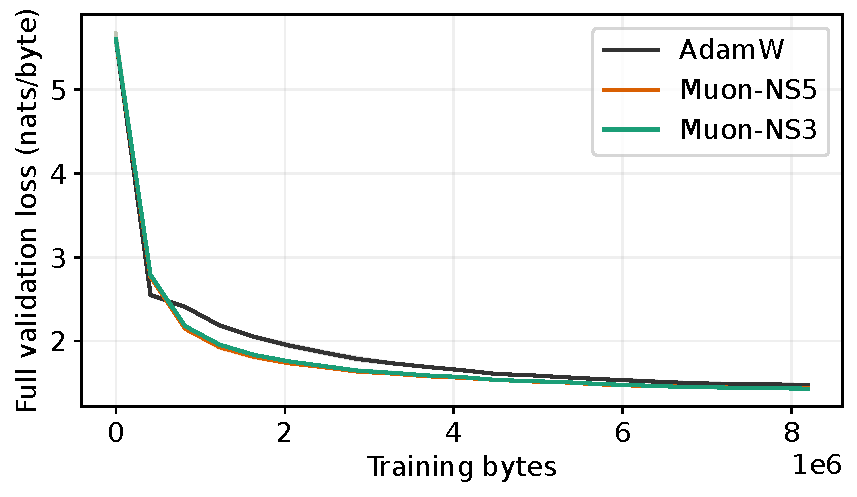
\includegraphics[width=.78\linewidth]{figures/language_bytes.pdf}
\caption{完整验证损失随训练字节数变化。实线为三种子的均值，阴影为样本标准差。}\label{fig:bytes}
\end{figure}
\begin{figure}[htbp]\centering
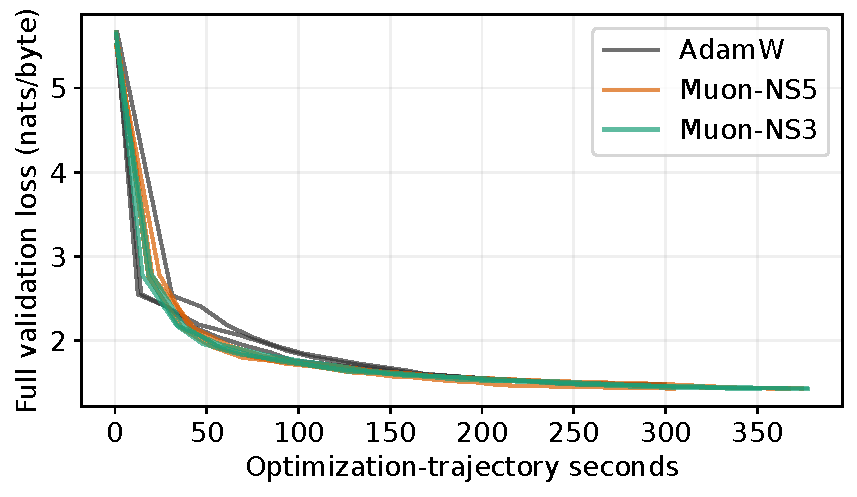
\includegraphics[width=.78\linewidth]{figures/language_time.pdf}
\caption{可恢复优化轨迹时钟下的验证损失，每条线为一个种子。此时钟不包含模型构建、末次保存或被回滚的工作，不能与表格累计任务时间混用。}\label{fig:time}
\end{figure}
NS5减去AdamW的三个配对测试损失差为-0.0285, -0.0525, -0.0532，平均差为-0.0447。
这说明在所列语料、模型和筛选预算下，NS5的平均测试损失较低；三个种子不足以支持跨模型规模或一般统计显著性的结论。
NS3复用了NS5的学习率，因而该比较考察固定设置下改变NS步数的效果，不代表为NS3单独调参后的最好表现。

\subsection{计算开销与适用范围}
正式GPU任务启动前整卡利用率范围为53\%至95\%，存在桌面图形负载。
任务间做垃圾回收与未使用CUDA缓存清理，记录的进程起始已分配量范围为16.25至16.25MiB。
表格和时间曲线是本机当次环境的观测，不用于宣称隔离环境的内核加速比。方法顺序按种子轮转，仍不能消除所有时变负载。
Tiny Shakespeare规模有限，且连续划分可能存在文本分布差异；本文采用字节编码与短上下文，不评价通用生成能力。
有限学习率网格、仅三个正式种子、辅助AdamW的固定学习率和精度设置都限制了结论范围。
完整理论假设未在该Transformer上验证；实际损失表现与单矩阵收敛证明应分别理解。
